%!TEX root = ../thesis.tex

\section{Evaluation}
To evaluate the capability and usability of \systemname{}, we conducted three user studies.
%
Since our motivation is to create illustrations that can be understood and learned, the first study with 10 participants tested the effectiveness of motion illustrations generated by \systemname{}.
%
The second study with the same 10 participants evaluated the \phaseI{} for recording and refining motion demonstrations.
%
The third study with 4 different participants evaluated the \phaseII{} for refining and editing a recording that was already captured.
%
We describe the details of each study with results in the sections below.

% ---------------------------------------------------------------

\begin{figure}[t]
  \centering
  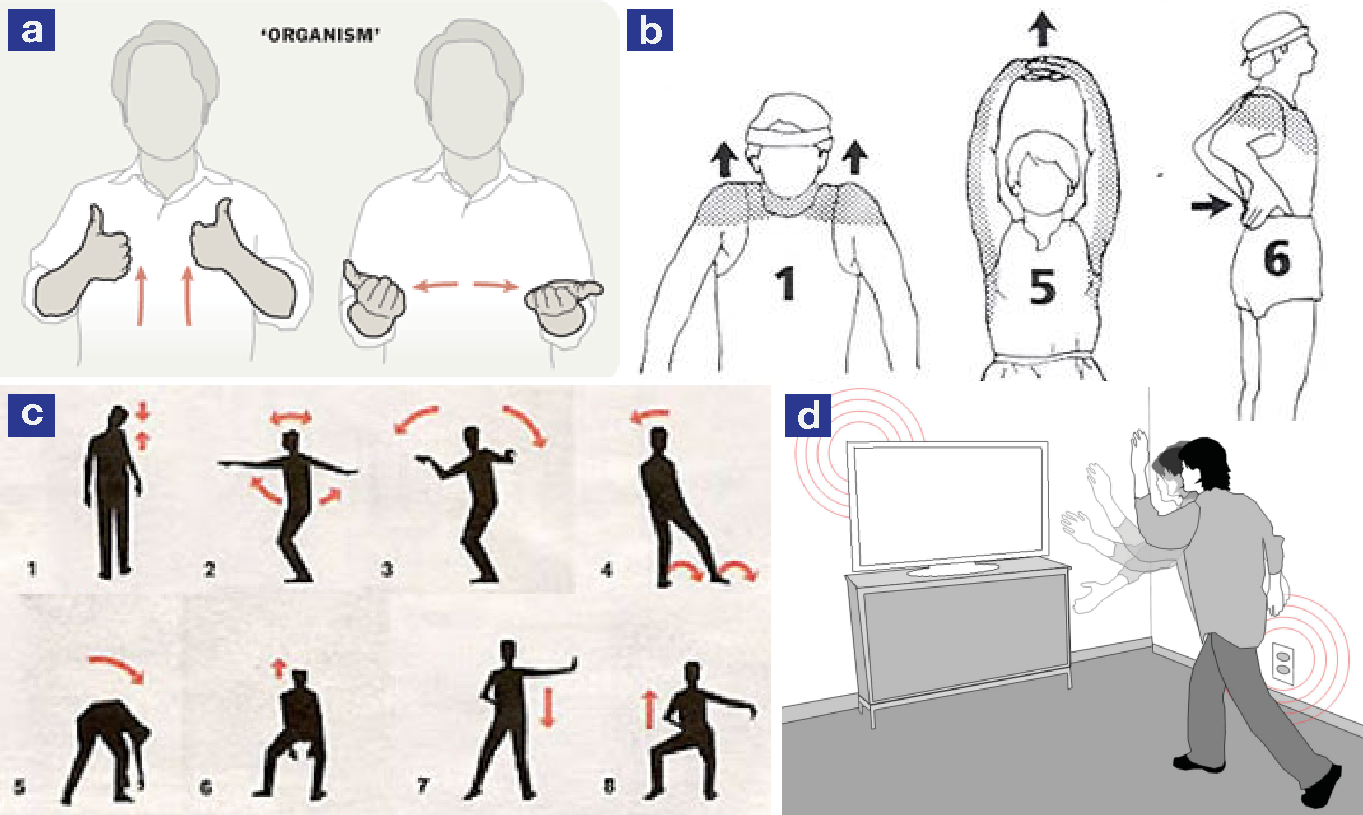
\includegraphics[width=0.8\columnwidth]{\demodraw/fig/existing_examples/existing_examples}
  \caption{Examples of manually generated movement diagrams from print and online materials for general audiences (a for sign language~\protect\cite{corum:2012:sign}, b for weight training~\protect\cite{anderson:2002:training}, c for Michael Jackson's Thriller dance moves [author unknown]); and from HCI publication (d for gestural interfaces~\protect\cite{cohn2012humantenna}).}
  % \dan{move this figure to evaluation, study 1 and show examples used in study}
  \label{fig:existing_examples}
\end{figure}

\subsection{Study 1: Illustration Effectiveness}

\subsubTitleBold{Hypothesis}
Learners with no prior experience can understand and re-perform motions after reviewing step-by-step illustrations generated by \systemname{}.

\subsubTitleBold{Participants}
We recruited 10 participants (5 females), aged 18 to 33 years (M=24.3), from a university and an IT company.
%
Six participants had previously created illustrations (from 5 to 50 diagrams), but none involved body motion. The common creation tool they used was Adobe Illustrator. %Four also had experience using 3D modeling software. %, including Blender, Unity, AutoCAD, and SolidWorks.
%
Among all participants, four were comfortable performing dance moves.

\subsubTitleBold{Experimental Setup}
The study was conducted in a lab environment with static indoor lighting.
%
A video camcorder was set up to record participants.

\subsubTitleBold{Procedure and Tasks}
To help introduce participants to the context of our work, we first provided existing examples of movement illustrations shown in Figure~\ref{fig:existing_examples}.
%
Then, we presented two sets of printed motion diagrams generated by the experimenters using \systemname{}. Each set included 4 steps (see Figure~\ref{fig:study_review_tasks}).
% \dan{which figure in the Appendix?}
For each set, we asked participants to interpret the illustrations and perform the depicted sequence in front of the camcorder when they were ready. %Illustration printouts were placed next to the video camera so that participants did not have to memorize the sequence.
%
On average, the study lasted 4 minutes; participants practiced one minute and half minute respectively for the two sets prior to recording.

\subsubTitleBold{Measures}
 We coded the video recordings as follows: for each joint movement in a step, we measured if 1) user intentionally moved the joint, i.e., a hit or a miss, 2) the start and end positions approximately matched the shown positions (e.g., moving right hand from lower left to upper right to the body), and 3) the movement from start to end positions was performed in the same way as shown (e.g., moving hand straight). We also marked if users intentionally moved other joints in addition to highlighted ones. We did not code the speed of each motion as our illustrations did not convey this element.
 \dan{what does ``measured'' mean? should this be ``assigned  a score out of X'' was it out of 3 marks? or 3 * number of joints moving? }

\subsection{Study 1 Results}
All participants successfully performed at least 5 of the 8 steps, with 10 of the 16 joint movements being correct (62.5\%). %For the remaining 6 movements in 3 steps, four were partially correct by 2-4 participants, one had an incorrect start position by 5 participants, and one was missed by 7 participants.
Table~\ref{tab:study1_errors} lists systematic errors made by our users and explanations they provided for them. Bi-directional arrows, motions involving independent trajectories of multiple body parts, following  complex trajectories, and inferring starting positions from arrows were all sources of errors. We suspect that some of the misinterpretations from our illustrations could be clarified via other visualization styles that \systemname{} is able to generate. We validate this in Study 3.

\begin{table}
  \centering
  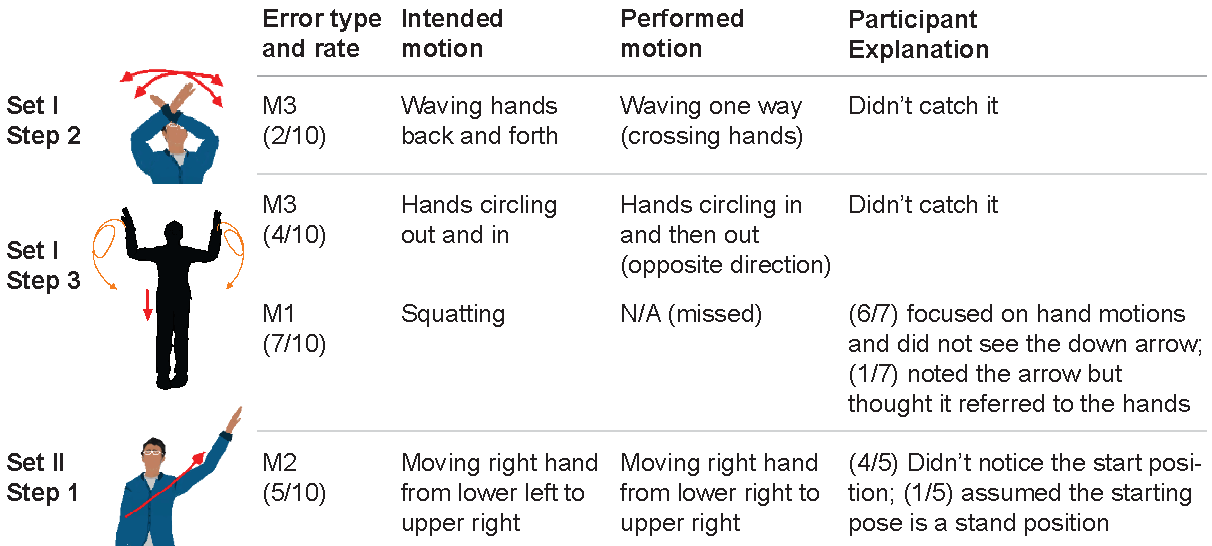
\includegraphics[width=\columnwidth]{\demodraw/fig/study1/study1}
  \caption{Incorrect movements performed by participants in Study 1.}
  \label{tab:study1_errors}
\end{table}

% ---------------------------------------------------------------

\subsection{Study 2: \phaseI{}}

\subsubTitleBold{Hypothesis}
Amateurs can efficiently create step-by-step motion illustrations using \systemname{}'s multi-modal \phaseI{}.

\subsubTitleBold{Participants}
The 10 participants from Study 1 completed this study immediately after the prior study.
%They were compensated with a \$15 gift card if they completed both studies.
Completing both study 1 and 2 took 45-60 minutes per participant.

\subsubTitleBold{Experimental Setup}
The study was conducted in the same space as Study 1. The \systemname{} system ran  on a Windows 8.1 machine, connected to a 30-inch monitor and external mouse and keyboard. The Kinect sensor was placed 3-feet above the floor to capture a 8$\times$8-feet clean office space.

\subsubTitleBold{Procedure and Tasks}
The study began with a learning phase where participants were introduced to \systemname{} and shown how to create the second set of illustrations from Study 1 by the experimenter.
%The experimenter recorded and reviewed the 4 moves twice.\bjoern{I don't understand what this sentence says - you performed the moves and recorded them into DemoDraw?}
Participants were then asked to record the same motions and review the results. This learning phase lasted 5-10 minutes.

Then participants completed an evaluation phase with four tasks in sequence:
\begin{enumerate}
  \itemsep -2pt
  \item The experimenter physically demonstrated a set of 4 moves for a gestural interface with the right hand, including waving, circling, making a reversed V shape, and swiping to the right (see~\ref{fig:study_authoring_tasks}-1). Participants were asked to record and review the captured results. Once they were satisfied with the recording, they were asked to rate each illustration step automatically generated by our syste,
  \item Similar to task 1, but with a set of 8 dance moves (see~\ref{fig:study_authoring_tasks}-2).
  \item The experimenter introduced the retaking operation and asked participants to choose one step from task 2 that they would like to revise. Participants re-performed part of the motion and reviewed.
  \item Participants were asked to perform any 4 to 8 moves they could imagine and retake them until they were satisfied with the results (within a time limit of 5 minutes).
\end{enumerate}
For each task, the numbers of attempts were not restricted.

\subsubTitleBold{Measures}
%
In tasks 1 and 2, participants rated each step along five dimensions: \iquote{Q1: The visualization accurately captured/described my motion} (a 5-point Likert scale from ``1: Strongly disagree'' to ``5:Strongly agree''), \iquote{Q2: The visualization shows all the important joints of movement}, \iquote{Q3: It shows at least one extraneous joint}, \iquote{Q4: The key pose was appropriately chosen} (Q2, Q3, and Q4 were answered ``Yes'', ``No'', or ``N/A''), and \iquote{Q5: This figure needs more (manual) editing before I would share it with others} (choose from ``1: Definitely needs edits'' to ``5: Very comfortable to share as is'').
\dan{this paragraph is pretty hard to read and understand}

An online questionnaire \dan{with additional questions?} was provided at the end of the study. Answers to both Likert-scale questions and comments were collected.
% \dan{Give some details about questions: how many questions? what were they about? what were the scales?}
% \peggy{I combined this in Discussion!}


\subsection{Study 2 Results}
On average, participants completed task 1 in 5 minutes with $\mu=2.3$ takes, task 2 in 10 minutes ($\mu=2.8$ takes), task 3 in 3 minutes ($\mu=2.3$ takes), and task 4 in 5 min ($\mu=2$ takes).
% General comments and observations you made about system performance.
\ref{fig:study_authoring_tasks} and~\ref{fig:open_ended_examples} provide examples of illustrations created by participants. Below we discuss participant feedback on the illustrations and the system design.

\subsubTitleBold{Ratings and Accuracy}
%We start from discussing the overall correctness of the results generated by \systemname{}.
% Figure~\ref{fig:ratings_graphs} shows the results specifically about accuracy and needs of editing.
Overall, participants thought the illustrations accurately described the motions (average median rating of 4.5 and 4.88
%M=4.23 and 4.66
% \bjoern{let's report medians not means for likert questions. Show the histograms in a small figure. Check the numbers, I guessed them.}
for task 1 and 2 respectively from Q1, where 5 = strongly agree), but on average, 4 of the 12 steps required further editing in order to share they illustrations with others (where medians were below 3 in Q5). Figure~\ref{fig:ratings_graphs} shows the results of step ratings.
%
P8 comments, \iquote{This figure represented the overall motion well (...) In particular, it captured all key poses, and the motion lines are easy to follow.} But P1 mentioned, \iquote{the system picked up really small movements in my other joints that were not relevant to the motion I was trying to depict (such as a small motion in my wrist or elbow).}
% \peggy{Question: put all the discussions in the later section? Like how we can improve our algorithm.}

\begin{figure}[t]
$\begin{array}{rl}
    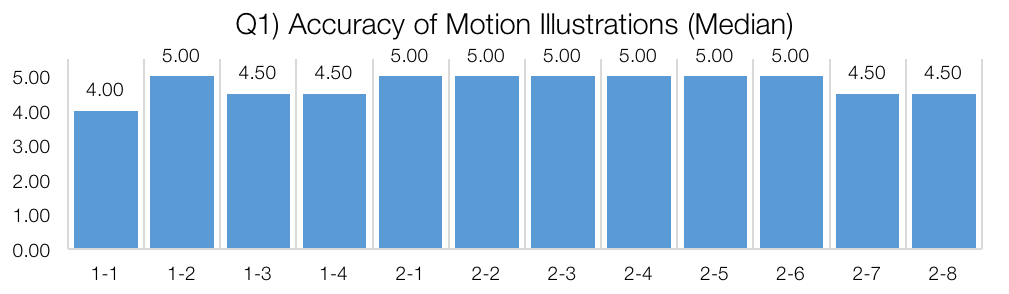
\includegraphics[width=0.7\columnwidth]{\demodraw/fig/study2/q1_accuracy}\\
    \multicolumn{2}{c}{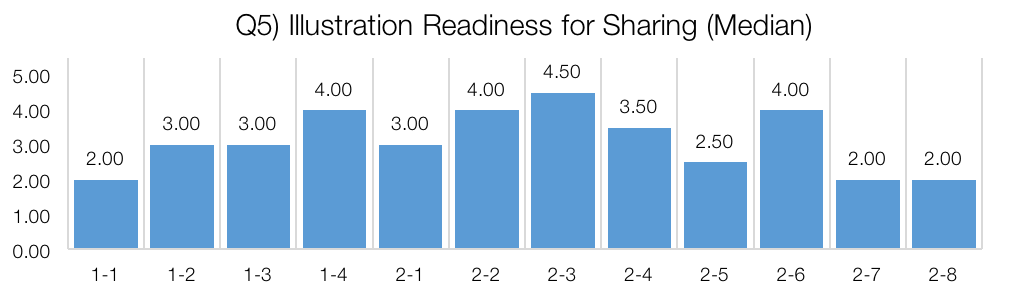
\includegraphics[width=0.7\columnwidth]{\demodraw/fig/study2/q5_editing}}
\end{array}$
\caption{User feedback from Study 2, showing the median rating of each step illustration.}
\label{fig:ratings_graphs}
\end{figure}

In the ratings of a total of 120 steps from 10 participants, all but one visualization (99\%) showed all the important joints (Q2), and in 80\% of cases the illustrations precisely selected only the salient joints without extraneous movements (Q3). Participants explained:
%
\iquote{the picture correctly represents my stance and body position. the arrows are easy to see and follow} (P1),
%
\iquote{the lines were very accurate} (P2), and
%
\iquote{The arcs are gorgeous and represent the intention of my motion really well.} (P5)
% \iquote{The figure represented the most important poses and movement directions.} (P8)
% \iquote{all of the motions were represented pretty accurately} (P1)



%\subsubTitleBold{Motion Capturing and Analysis}
%Participants were satisfied with our automatic techniques on visualizing their demonstration (M=4.2 and 4.6 for task 1 and 2 respectively in a 5-point Likert scale). They commented:
%\iquote{I'm impressed that the system captured the back and forth of my wave} (P5) and
%\iquote{Swiping motions, making a circle. When it gets the motion, it gets it perfectly} (P7) for task 1.
%Segmentation results were also positive:
%\iquote{Most of the time, the arrows are only attached to key joints that move} (P2).
%
Several participants mentioned that they appreciated how \systemname{} smoothed the arrows, especially when their demonstration was not perfect or there was some capture noise.
% \bjoern{Is this smoothing discussed anywhere in the paper? If not, cut it.} in pipeline
%
Some noted the motion data capturing in 3D as an advantage.
During the debrief session, some participants were shown the illustrations from different view points as their motion involved changes in depth. As P9 noted: \iquote{I love the multiple camera angles for the wiggle arm motion I did in step 1.}
% \iquote{I also liked that in most steps the arrows were only on the key motions, and all of the motions had smooth arrows.} (P8)

\subsubTitleBold{Key Pose Selection}
Participants found 94\% of key poses were selected correctly (Q4), commenting for example:
%\iquote{It does a great job with the key poses!} (P3),
%\iquote{This figure captured the key poses perfectly} (P8),
%\iquote{All of the key poses in the 8 figures are chosen wisely} (P10),
\iquote{The key poses are very descriptive of the motion} (P2), and
\iquote{The key frames were just right} (P5).
%
% These show that

\subsubTitleBold{Authoring Workflow}
Participants found it easy to learn \systemname{} (Median=5 out of 5) and easy to create illustrations using our system (Median=4.5).
% \bjoern{again report median and show histogram}
%P9 liked our system as it was \iquote{fast and easy to use; just demonstrate and the motion is captured}, and
%P4 \iquote{was super excited to get great results on my first take.}
%
%We believe that the multi-modal interaction design is suitable for a motion-driven application like \systemname{}.
All participants were able to author and navigate via the speech interface.
Specifically, P10 noted, \iquote{The voice command allows people be able to control the system remotely. Without the voice capability, the system can be impractical in the single-person use case.}

Participants were especially impressed by how fast authoring could be to generate a step-by-step diagram:
\iquote{Surprisingly fast to make some really cool full-body motion demonstrations. There is no way I could do this in higher-fidelity than a napkin sketch in the same time} (P5) and
\iquote{the system saves significant amount of time creating illustrations} (P10).
%
We also asked participants to estimate the time required if they were to generate a similar 8-step diagram without using \systemname{}, four participants answered that they would not be able to create manually, while others responded that it would take 90 to 160 minutes as each single figure might take 10-20 minutes.
%
%\iquote{Using illustrator alone, I wouldn't be able to create these types of illustrations but using this system I can} (P8),
%\iquote{it was much faster, and you didn't need any photo editing experience to create your own illustrations} (P1), and
%\iquote{Can get a lot of work down in a relatively small amount of time compared to other systems} (P6).
% \iquote{Very quick and efficient. And then can edit post-recording to make it look nice. Can get a lot of work down in a relatively small amount of time compared to other systems.} (P6)

\subsubTitleBold{Improving a Demonstration}
The immediate visual feedback during the capturing phase was effective in helping authors review, adjust, and retake their performances.
P4 explained, \iquote{I learned how to exaggerate the important aspects of motion without being explicitly told to.}
%This was also observed from most participants as they adjusted the motions and re-performed the motions after playing back the illustrations.
In task 3, when we introduced the retaking capability, participants explained that this function would be especially helpful for a long motion sequence. All but one participant chose to retake step 2-7, which involved a holding position with one foot. %Instead of redoing the six steps beforehand, they redid step 2-7 and 2-8 several times (M=2.3 takes).
Three participants later used the same technique for task 4. P8 also noted that it was helpful as \iquote{I could improve this by retaking that step and moving smoothly} when referring to a specific pose that she thought needed additional work.
% \iquote{it was fun.} (P9)
% \iquote{So much easier, smaller barrier of entry } (P7)
% \iquote{I like these illustrations because the focus of the diagram is on the motion.} (P8)

% Table X shows median ratings for the 5 accuracy-related questions for each tasks.
% \dan{the only statistical test I could imagine useful would be comparing whether retake improved the rankings -- if it didn't, then the system is good to start, if it did, then the retake function works and is important.}
% Overall, the system performed well.
% Participants were less satisfied with blah and blah, especially in task X.
% The higher scores for task 3, the retake step, demonstrate the importance of this feature.
% \dan{some kind of commentary and what you saw, main result should be system worked and people could generally capture what they wanted.}

% ---------------------------------------------------------------

\subsection{Study 3: \phaseII{} Effectiveness}

To understand how users refine automatically-generated results and generate different visualization styles in \systemname{}'s \phaseII{}, we conducted an informal study with 4 participants (all males, aged 23 to 32 years, M=28) from an IT company.
%
The same experiment setup as Study 2 was used.
%and \$15 compensation as Study 2 was used.

% \subsubTitleBold{Procedure and Tasks}

% We provided example illustrations and walked through a warm-up task.
% , including a sign language guide, an airline safety guide, and a Kinect game tutorial
We provided a warm-up task where participants loaded one motion recording, which showed a continuous movement of lifting the right hand up and pushing to the right. Experimenters guided them to create an illustration with a thick arrow showing the hand movement using \systemname{}. Manipulations included the motion segmentation boundary, selecting joints of interests, line width and color, visual styles, and viewpoints. This learning phase was 5 minutes on average.

Four tasks were given in sequence:
% To evaluate if our system could support both creating specific illustrations and designing user-generated motions, we designed two parts of a study:
% included two types of tasks: 1) Given an illustration of a motion capture file captured and created by the authors, approximate the illustration with \systemname{}, and 2) given a movement specified by the experimenter in front of the participants, physically record and create an illustration using \systemname{}'s authoring UI.
%
In tasks 1 and 2, participants were given a motion recording and three illustrations created using our system. We presented the printed figures one by one and asked them to approximate them with \systemname{}.
% Task 1 showed a motion of two hands waving in opposite directions, which involved two joints and change of default arrow style. Task 2 showed a motion that a person squat down after circling two hands, which involved multiple joints (two with relative positions) and change of camera viewpoint.
%
% \dan{Would it be better to write tasks asking for an illustration style, rather than requiring a specific UI function? Task 1: illustrate a two armed side wave (requires two two-headed arrows, possibly overlay)}
%
In tasks 3 and 4, participants used \systemname{} to physically perform and record two specific motions that experimenters introduced.
% Experimenters helped hit the record button when they indicated that they were ready.
They then used our system to create an illustration that they thought would best convey the motion. They were free to use any skills they had learned from the previous tasks without time limitation.
%
Finally, an online questionnaire was provided.
% \dan{Give some details about questions: how many questions? what were they about? what were the scales?}


\subsection{Study 3 Results}

% All the participants successfully completed the tasks and created illustrations. (see Figure~\ref{fig:study3_results} for selected examples).
%
%Similar to Study 2, participants found it easy to learn (M=4.25 out of 5) and create a motion illustration (M=4.5) using \systemname{}. P1 commented that it was \iquote{Super easy to use and create different illustration styles quickly}, and P3 thought, \iquote{the fact that you can change up the colors and characters is a cool bonus!}
%
Unlike Study 2, which used only one illustration style with motion arrows, this study provided more versatile visualization techniques and manual refinement. We noted that participants actively tweaked visual parameters and the styles using the available options from the \phaseII{}, especially when creating the stroboscopic effect. Decisions include: numbers of intermediate frames and the layout, dragging to reposition the arrows, and arrow color and width.
% \bjoern{not sure what you mean by ``rather than specific joint movements" - what did they not do?}
%
In addition, participants had strong preferences on styles once they had several visualization options. For example, P4 explicitly commented on the stroboscopic effect of task 3 as \iquote{this is exactly what I looked for -- It clearly conveys the start and end poses.} P2 preferred the cartoon renderer than silhouette as \iquote{this character looks just like me!}
%
They indicated that they were not able to create similar illustrations without using \systemname{} (Median=2).
%
These results indicated that the detailed editing aspect of our system through the \phaseII{} was effective in authoring illustrations that could be expressive for various types of motions.

\begin{figure}[t]
  \centering
  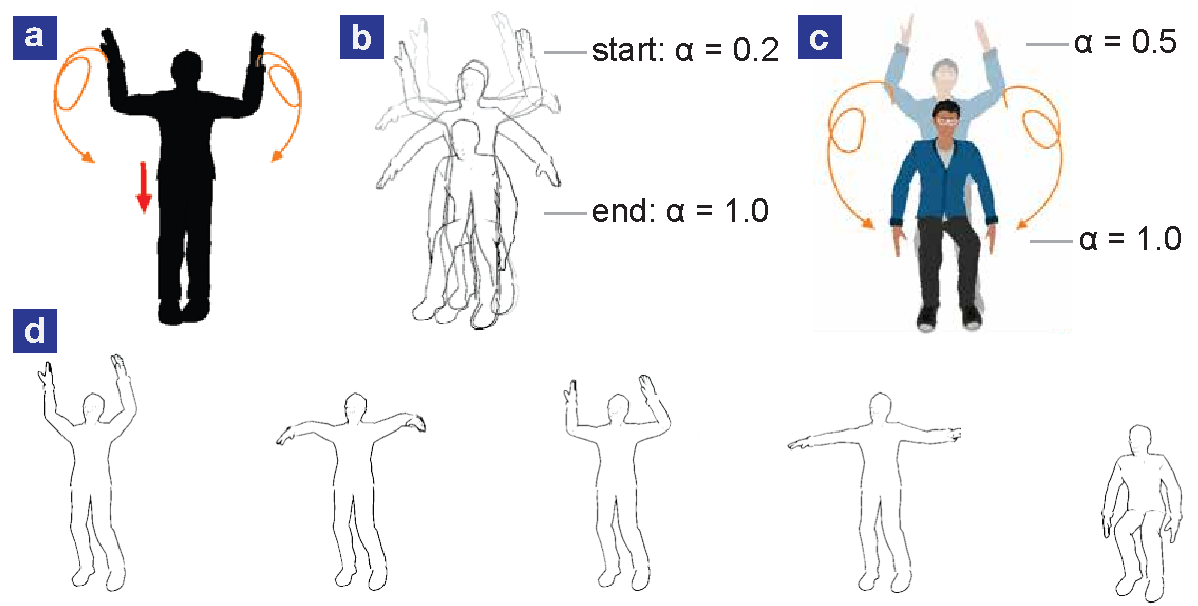
\includegraphics[width=0.8\columnwidth]{\demodraw/fig/study3/study3_effects}
  \caption{Different illustration effects conveying the same motion recording using \systemname{}'s \phaseII{}: a and c are created by the paper authors and a was used in Study 1; b by Study 3-P1 using 4 intermediate frames with zero offset; d by Study 3-P2 using 5 frames, positioned as a sequence.}
  \label{fig:study3_effects}
\end{figure}


% P4 commented, \iquote{figures themselves looked very accurate.}
%
% We measured the quantitative user performance and collected qualitative user feedback. In particular, for each task, we logged the total time of completing a task (from loading a recording to finish), number of edits (any adjustment of parameters), and number of similar attempts (if an operation was executed more than one time continuously). We also observed their high-level strategy of creating an illustration.

% \begin{figure}[t]
%   \centering
%     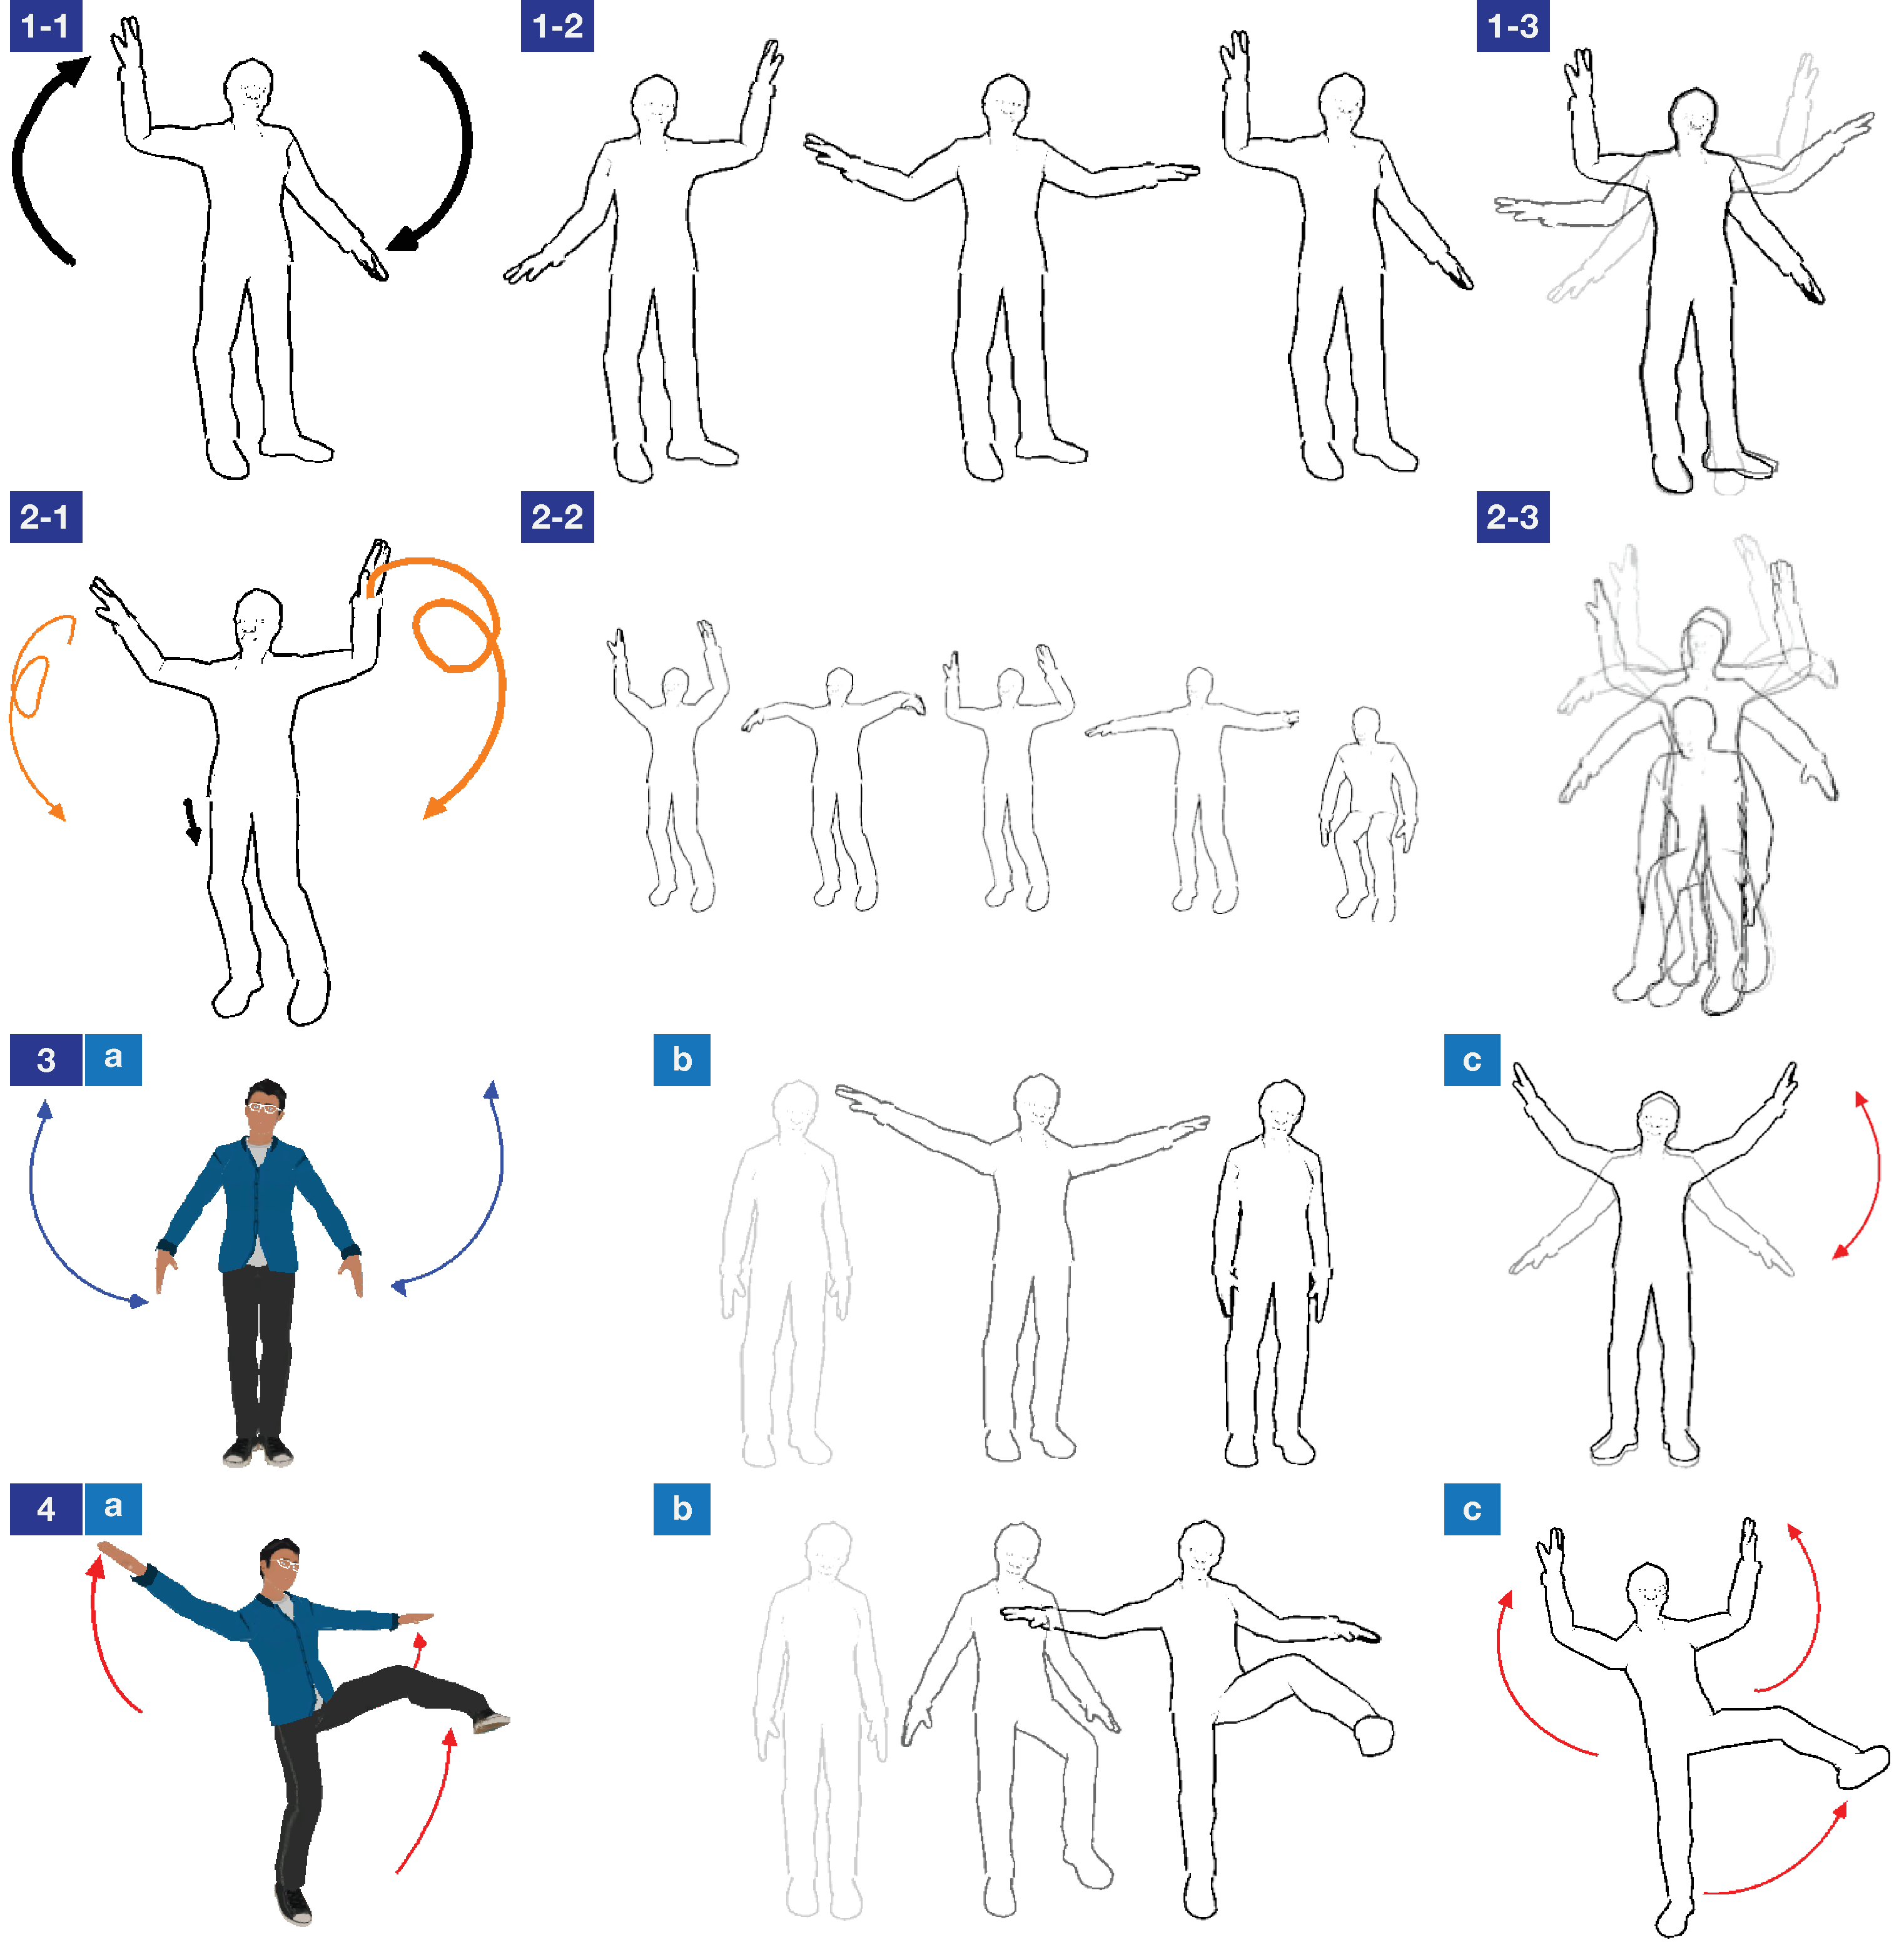
\includegraphics[width=\columnwidth]{fig/study_tasks}
%   \caption{Illustrations created by different participants in Study 3.}
%   \label{fig:study3_results}
% \end{figure}
